\title{2020/03/27 Discussion}
\author{0616014 楊政道}
\maketitle
\thispagestyle{fancy}
\section{Discussion 1}
\subsection{Based on the requirements, set correct value in the sample code}
\begin{itemize}
    \item Output data rate: 100Hz
    \item $\pm$ 2g
    \item Convert LSB to G (by using SCALE\_MULTIPLIER)
\end{itemize}
\begin{figure}[!h]
    \begin{center} 
        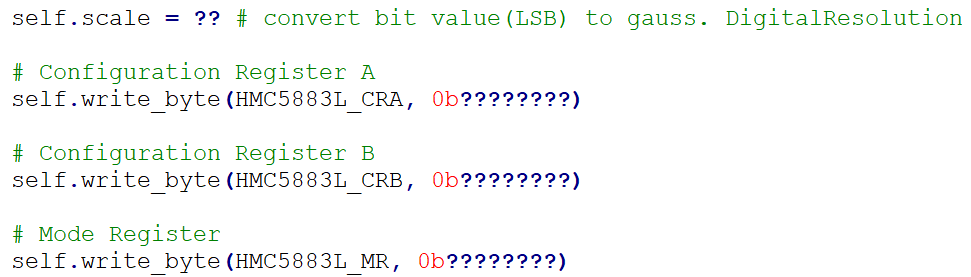
\includegraphics[width=10cm]{d1-1.png} 
    \end{center} 
\end{figure} 
\subsubsection{ADXL345\_SCALE\_MULTIPLIER}
\paragraph{}
The value of the \texttt{ADXL345\_SCALE\_MULTIPLIER} is \texttt{1/SENSITIVITY}. According to the datasheet, the value of the sensitivity is \texttt{256 LSB/g}. Therefore, the value of the \texttt{ADXL345\_SCALE\_MULTIPLIER} is \texttt{1/256=0.00390625}.
\begin{figure}[!h]
    \begin{center} 
        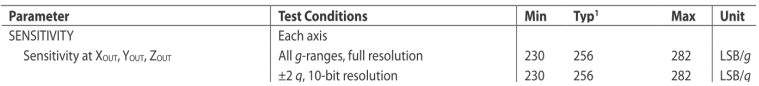
\includegraphics[width=10cm]{d1-1_datasheet-1.png} 
    \end{center} 
\end{figure} 
\subsubsection{ADXL345\_BW\_RATE\_100HZ}
\paragraph{}
The value of the \texttt{ADXL345\_BW\_RATE\_100Hz} is a 8-bit integer value. According to the datasheet, we can find the rate code is \texttt{1010} if we want the output data rate is \texttt{100Hz}. Therefore, the value of the \texttt{ADXL345\_BW\_RATE\_100HZ} is \texttt{0x0A}.
\begin{figure}[!h]
    \begin{center} 
        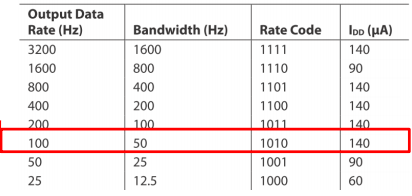
\includegraphics[width=5cm]{d1-1_datasheet-2.png}
    \end{center}
\end{figure}
\newpage
\subsubsection{ADXL345\_MEASURE}
\paragraph{}
The value of the \texttt{ADXL345\_MEASURE} is to set the \texttt{ADXL345} into measure mode. According to the datasheet, we can set the \texttt{POWER\_CTL} register into {00001000}. Therefore, we will set the ADXL345 into measure mode.
\begin{figure}[!h]
    \begin{center} 
        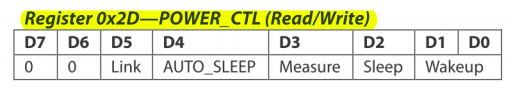
\includegraphics[width=10cm]{d1-1_datasheet-3.png} 
    \end{center} 
\end{figure} 
\subsection{Continuously measurement}
\paragraph{}
\begin{figure}[!h]
    \begin{center} 
        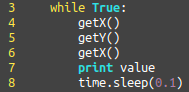
\includegraphics[width=5cm]{d1-2_structure.png} 
    \end{center} 
\end{figure} 
\paragraph{}
The sample code can only output the value once. If we want to measure continuously, we can put the sample code into a while loop with a sleep statement.
\subsection{Calibrate your sensor}
\paragraph{}
Set all the offsets value into zero and output the value read from sensor.
\begin{figure}[!h]
    \begin{center} 
        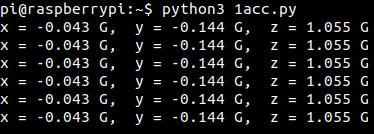
\includegraphics[width=10cm]{d1-3_before.png} 
    \end{center} 
\end{figure} 
\paragraph{}
The value read from the sensor should be (0, 0, 1) theoretically, so we need to set the offsets to make the value into correct ones.
\begin{figure}[!h]
    \begin{center} 
        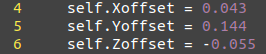
\includegraphics[width=10cm]{d1-3_set-offset.png} 
    \end{center} 
\end{figure}
\newpage
\paragraph{}
After we set the offset value, the output will close to (0, 0, 1).
\begin{figure}[!h]
    \begin{center} 
        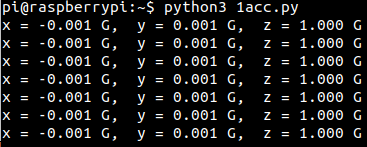
\includegraphics[width=10cm]{d1-3_after.png} 
    \end{center} 
\end{figure} 
\section{Discussion 2}
\subsection{Based on the requirements, set correct value in the sample code}
\begin{itemize}
    \item Data rate: 100Hz, cut-off = 12.5
    \item Full Scale selection = 250 dps
    \item Set Sensitivity for 250 dps (by using SCALE\_MULTIPLIER)
\end{itemize}
\begin{figure}[!h]
    \begin{center} 
        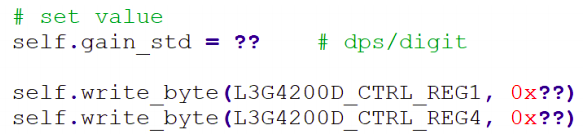
\includegraphics[width=10cm]{d2-1.png} 
    \end{center} 
\end{figure} 
\subsubsection{gain\_std}
\paragraph{}
Since the sensitivity is 8.75 mdps/digit, the value of the \texttt{gain\_std} will be \texttt{8.75$\times 10^{-3}$ = 0.00875}.
\newpage
\subsubsection{L3G4200D\_CTRL\_REG1}
\begin{figure}[!h]
    \begin{center} 
        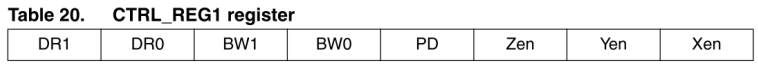
\includegraphics[width=8cm]{d2-1_datasheet-1.png} 
    \end{center} 
\end{figure} 
\begin{figure}[!h]
    \begin{center} 
        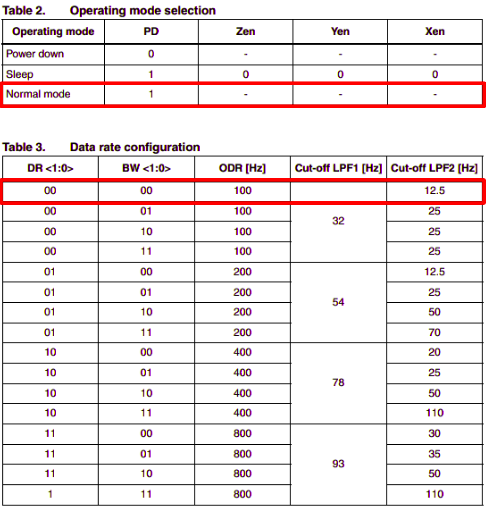
\includegraphics[width=8cm]{d2-1_datasheet-1-detail.png} 
    \end{center} 
\end{figure} 
\paragraph{}
According to the datasheet, we need to set \texttt{L3G4200D\_CTRL\_REG1} into 0x0F so as to make data rate 100Hz, cut-off rate 12.5 and the sensor into normal mode.
\subsubsection{L3G4200D\_CTRL\_REG4}
\begin{figure}[!h]
    \begin{center} 
        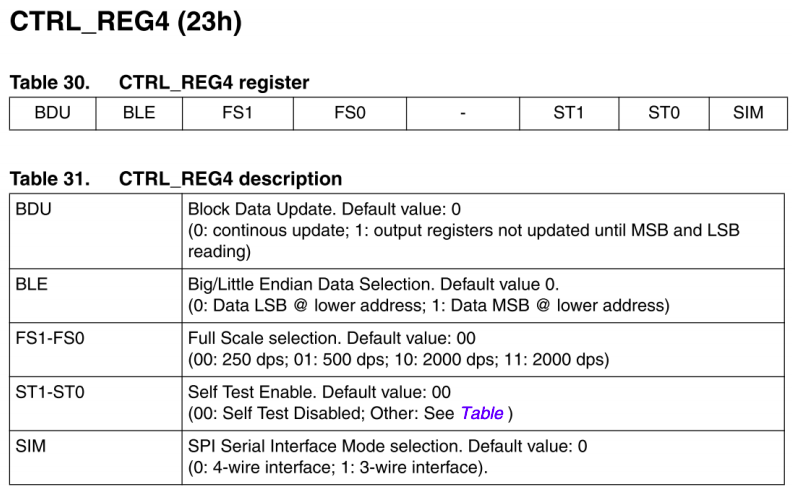
\includegraphics[width=8cm]{d2-1_datasheet-2.png} 
    \end{center} 
\end{figure}
According to the datasheet, we need to set all the bits, except the reserved one, into zero. Therefore, we can match the requirements mentioned above. (There is a typo in the equation at page \texttt{36} of the slide, \texttt{0x80 = 0000 1000}. It might be 0x08).
\newpage
\subsection{Continuously measurement}
\paragraph{}
\begin{figure}[!h]
    \begin{center} 
        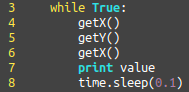
\includegraphics[width=5cm]{d1-2_structure.png} 
    \end{center} 
\end{figure} 
\paragraph{}
The sample code can only output the value once. If we want to measure continuously, we can put the sample code into a while loop with a sleep statement.
\section{Discussion 3}
\subsection{We can obtain ax/ay/az from accelerometer. How to calculate the distance?}
\paragraph{}
First, we can calculate the distance in 3 dimensions separetely, and then combine this 3 data into a real distance by the below equation.
$$D = \sqrt{{D_x}^2 + {D_y}^2 + {D_z}^2}$$
\paragraph{}
We can draw the a-t plot first.
\begin{figure}[!h]
    \begin{center} 
        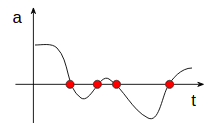
\includegraphics[width=10cm]{d3_at.png} 
    \end{center} 
\end{figure}
\paragraph{}
Then, we can construct the v-t plot. The value \texttt{v(t)} at \texttt{t} on the v-t plot is the area from zero to \texttt{t} on the a-t plot, as known as integration.
\begin{figure}[!h]
    \begin{center} 
        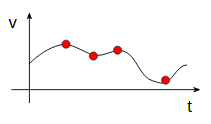
\includegraphics[width=10cm]{d3_vt.png} 
    \end{center} 
\end{figure}
\paragraph{}
Therefore, if we want to calculate the distance, we can calculate the area on the v-t plot. The equation wil be like below one.
$$D_x = \int_{0}^{t} (\int_{0}^{t} a_x(t) dt) + v(0) dt$$
\paragraph{}
Similar to the $D_y$ and $D_z$
$$D_y = \int_{0}^{t} (\int_{0}^{t} a_y(t) dt) + v(0) dt$$
$$D_z = \int_{0}^{t} (\int_{0}^{t} a_z(t) dt) + v(0) dt$$
\paragraph{}
For the implementation, we will split the area into many pieces. For each piece, we can treat it as a uniform accelerated motion and use the formula below to calculate the distance.
$$s = v_0t + \frac{1}{2}at^2$$
\paragraph{}
So the result will be
$$D_x = \sum_{i=0}^{n-1}{v_x(\frac{it}{n})\frac{t}{n}+\frac{1}{2}a_x(\frac{it}{n})(\frac{t}{n})^2}$$
\paragraph{}
Similar to the $D_y$ and $D_z$
$$D_y = \sum_{i=0}^{n-1}{v_y(\frac{it}{n})\frac{t}{n}+\frac{1}{2}a_y(\frac{it}{n})(\frac{t}{n})^2}$$
$$D_z = \sum_{i=0}^{n-1}{v_z(\frac{it}{n})\frac{t}{n}+\frac{1}{2}a_z(\frac{it}{n})(\frac{t}{n})^2}$$
